\section{数据探索与规律发现}

本章把全部可观察到的数据规律逐一列出，并\textbf{逐条给出建模决策}：能够带来成本改进的规律
显式写入模型（第 5--8 节）；不单独建模的规律同样给出“数据 + 图表”的理由，避免“拍脑袋取舍”。

\subsection{数据总览与质量核验}

\begin{table}[htbp]
\centering
\caption{数据质量核验结果（清洗前后）}
\label{tab:quality}
\small
\begin{tabular}{@{}lllll@{}}
\toprule
数据 & 原始形态 & 缺失 & 负值/重复 & 清洗后 \\
\midrule
附件1 & 144$\times$4（区间结束时刻标签） & 0 & 0 / 0 & 长表 144 行（slot 1--144） \\
附件2 负载 & 365$\times$145（宽表） & 0 & 0 / 0 & 长表 52\,560 行 \\
附件2 光伏 & 365$\times$145 & 0 & 0 / 0 & 长表 52\,560 行 \\
附件3 预报 & 1460$\times$26 & 1095（结构空值） & 0 / 0 & 向下填充；35040 行绝对小时映射 \\
附件4 电价 & 365$\times$145 & 0 & 0 / 0 & 长表 52\,560 行 \\
\bottomrule
\end{tabular}
\end{table}

统一时间轴为 $(date,slot)$：日期取 2025-01-01 至 12-31 共 365 天，$slot=1,\dots,144$
对应区间 $[(slot-1)\times10,\,slot\times10)$ 分钟。功率（kW）与电量（kWh）的换算是
$1\ \text{kWh}=\text{kW}\times\frac{10}{60}\ \text{h}$。附件3 的预报口径经实测校验为
“发布时刻后第 $k$ 个整点的功率点”（如 0:00 发布的“预报 7 小时”=3.12 kW 对应 7:00 实测 3.08 kW），
故用\textbf{整点功率点 + 线性插值}细化到 10 分钟。

\subsection{规律一：周内负荷规律（周五、周六显著偏低）}

按星期统计日均用电量：周一至周四与周日均为 123.9--124.9 MWh/日，而\textbf{周五 78.3 MWh、
周六 78.4 MWh，比其他五天低 36.8\%}（\cref{fig:weekly} 左上）。该规律在 12 个月中全部成立，
是“昨日外推”预测的最大误差来源：若用周四实测预测周五，负荷被系统性高估约 46\%。

\textbf{建模决策（已建模，并进一步升级）}：0:00 计划依据先改为“\textbf{近 4 个同类日
（周五六 / 其他五天两类）实测平均}”（负载 MAE 由昨日外推的 108.3 降到 22.9 kWh/时段），
再升级为第 \ref{sec:q2} 节的“\textbf{水平$\times$形状分解 $+$ 分类凸组合}”模型：
负载 MAE 进一步降至 \textbf{22.0 kWh/时段（132.3 kW）}，
其中\textbf{周五、周六由 154.6 kW 降到 142.2 kW（$-8.0\%$）、其余五天由 130.7 降到 128.3 kW（$-1.8\%$）}；
全年（2.1--12.31）购电总费用由 21\,491\,755 元降至 \textbf{13\,655\,835 元（节约 36.5\%）}。

\subsection{规律二：周内电价规律（周五、周六显著偏低）}

附件4 实时电价同样呈现周内规律：\textbf{周五 0.6290、周六 0.6298 元/kWh，比其他五天
（0.8191--0.8238）低 23.3\%}，且 12 个月逐月一致（\cref{fig:weekly} 左下），
白天时段价差最大（8 时低 0.33 元/kWh）。由于周几的判定必须精确，这里给出日历实锤
（\cref{tab:calendar}）：全年日均电价最低的 10 天全部为周五或周六（最低的
2025-04-26 为周六、0.5378 元/kWh），而 2025-01-05（周日）为 0.9252 元/kWh 属于高价日。

\begin{table}[htbp]
\centering
\caption{周内电价规律的日历验证（2025 年 1 月第一周）}
\label{tab:calendar}
\small
\begin{tabular}{@{}lccccccc@{}}
\toprule
日期 & 01-01 & 01-02 & 01-03 & 01-04 & 01-05 & 01-06 & 01-07 \\
星期 & 周三 & 周四 & \textbf{周五} & \textbf{周六} & 周日 & 周一 & 周二 \\
日均电价(元/kWh) & 0.9265 & 0.9266 & \textbf{0.7386} & \textbf{0.7303} & 0.9252 & 0.9290 & 0.9234 \\
\bottomrule
\end{tabular}
\end{table}

\textbf{建模决策（不单独建模）}：问题四假设“规划时已知当日实时电价”（对应现货日前市场口径），
LP 逐时段使用真实电价，\textbf{周内规律已被最优解自动利用}。证据：采用方案中各星期日均充放电量
显示，周四净充电仅 $+2592$ kWh（全周最低，为周五低价让路），而\textbf{周五净充电
$+5622$ kWh（全周最高）}。稳健性检验：即使 0:00 不知道当日电价、改用
“类别$\times$时段廓线 + 自适应水平 + GBDT 堆叠”的电价预测模型（MAE $=0.0367$ 元/kWh）
制定计划、结算仍按实际电价，全年费用反而\textbf{降低} 28\,175 元（$-0.20\text{\%}$），
说明结论对电价信息假设稳健，且该发现提示“计划阶段过度追价会损害日内兜底能力”。

\subsection{规律三：光伏季节特征（强季节 + 雨季凹陷）}

月度日均光伏电量由 12 月的 36.3 MWh 上升到 8 月的 70.0 MWh，\textbf{最高/最低 $=1.93$ 倍}；
年周期正弦拟合 $E=A+B\sin[2\pi(d-\varphi)/365]$ 得 $R^2=\textbf{0.754}$、振幅 14.2 MWh
（年均值的 25.6\%）、峰值日约 7 月 1 日；数据代理的“有效日照时长”冬季 10.0 h/日、
夏季 12.9 h/日，与日光伏电量相关系数 0.855；四季日曲线形态（日出日落时刻与正午峰值高度）
差异明显。此外，\textbf{6 月出现“雨季凹陷”}（56.9 MWh，低于 5 月的 67.4 与 7 月的 65.4），
说明季节特征由天文因素与气候因素叠加，偏离纯正弦（\cref{fig:pvseason}）。

\textbf{建模决策（不单独建模），三层证据}：
\begin{enumerate}[label=(\arabic*), leftmargin=2.2em, itemsep=1pt]
\item \textbf{直接试验}：在基值上叠加“季节动量趋势”（爬坡期自动上调、下降期自动下调）后，
全年费用上升 \textbf{0.63\%}（+85\,264 元）——动量项把天气噪声误当作趋势放大；
\item \textbf{残差偏置检验}：光伏基值（近 4 日均值）的逐月误差均值全年仅 $-0.34$ kWh/时段、
任何月份不超过 $\pm7$ kWh/时段（相对标准差 27--67 可忽略）；负荷侧同理（全年 $-0.58$）。
即基值\textbf{已无季节系统偏差}；
\item \textbf{缓冲层检验}：按“上月调优、当月使用”的逐月滚动重调报童分位，
全年费用 13\,836\,136 元，仅比常数 $q^*=0.7$ 低 0.09\%（12\,046 元），
且逐月选出的 $q^*$ 在 0.7 与 0.8 之间无规律跳动（\cref{tab:buffer}），
说明\textbf{最优缓冲水平不随季节变化}。
\end{enumerate}

\begin{figure}[htbp]
\centering
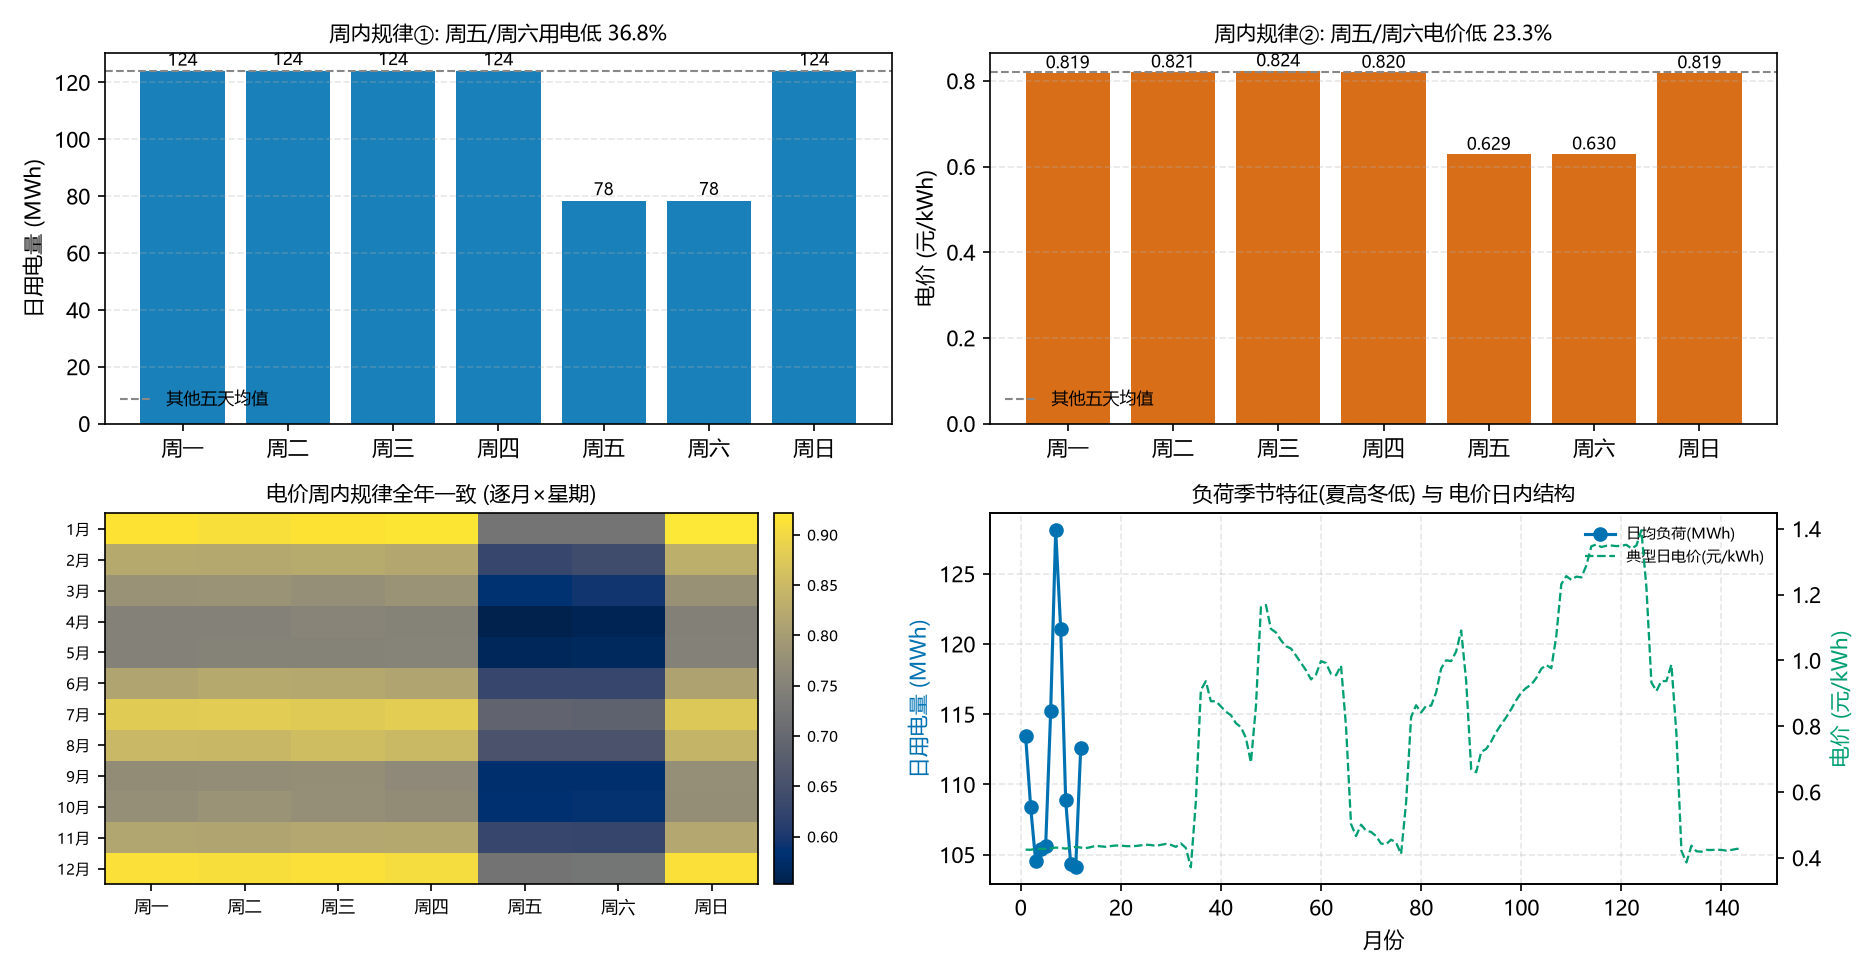
\includegraphics[width=0.92\textwidth]{figures/fig_weekly.png}
\caption{周内规律：日均用电量（左上）、日均电价（右上）、逐月$\times$星期电价热力图（左下）、
负荷季节特征与电价日内结构（右下）}
\label{fig:weekly}
\end{figure}

\begin{figure}[htbp]
\centering
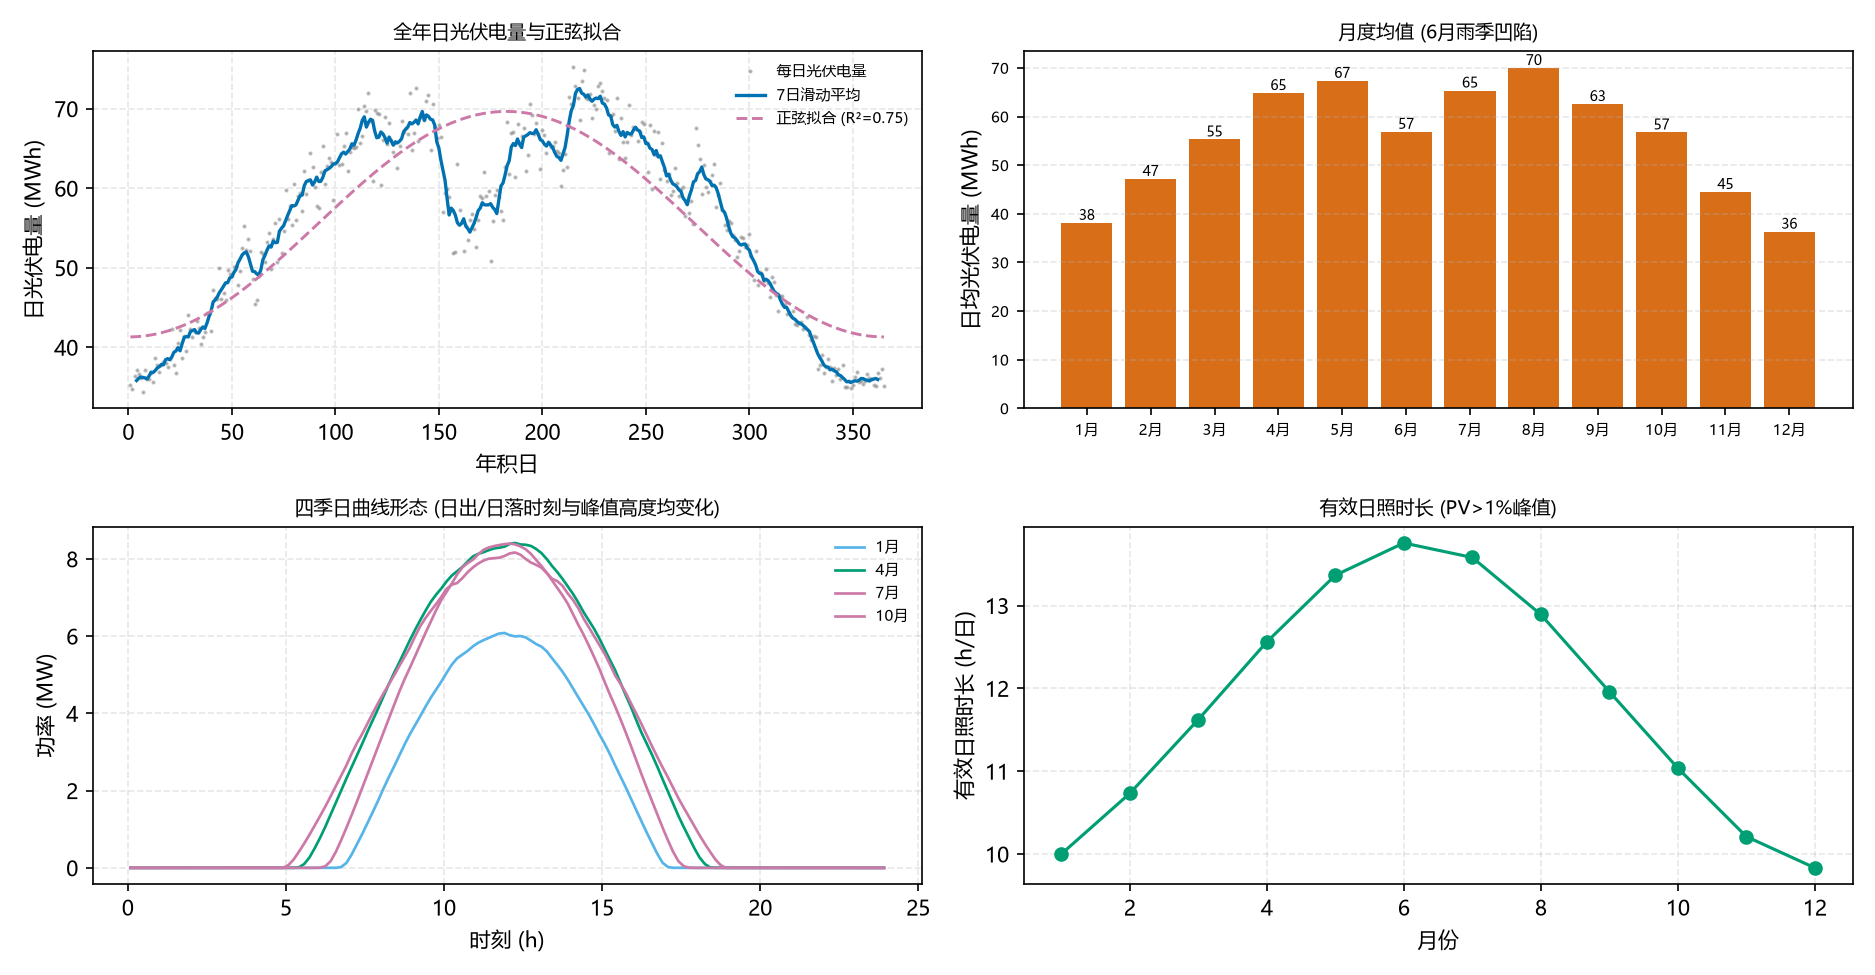
\includegraphics[width=0.92\textwidth]{figures/fig_pv_season.png}
\caption{光伏季节特征：全年日电量与正弦拟合（左上）、月度均值与雨季凹陷（右上）、
四季日曲线形态（左下）、有效日照时长（右下）}
\label{fig:pvseason}
\end{figure}

\subsection{规律四：光伏与负荷噪声的重尾特征}

以“近 4 个同类日平均/近 4 日均值”为基值，净需求残差 $e=e_L-e_P$ 的分布呈现明显
\textbf{重尾}：偏度均值 $+0.16$（近似对称），而\textbf{超额峰度均值 $+5.96$}（正态为 0，
个别时段高达 21）；标准差最大出现在 12 时（112.2 kWh/时段），与正午光伏波动一致。
按月看，光伏基值误差的标准差在春季与雨季最大（MAE 31--35 kWh/时段），12 月最小（12.9）。

\textbf{建模决策（已建模：经验分位缓冲；并证明“形式不重要、水平才重要”）}：安全裕度取
\textbf{近 30 天净残差的 70\% 经验分位}。五组对照实验（\cref{tab:buffer}）显示：
各种更复杂的形式与本文方案的差异都在 $\pm0.6\text{\%}$ 以内
（分噪声叠加 $-0.52\text{\%}$、正态参数化 $+0.58\text{\%}$、60/90 天长窗 $+0.03$/$+0.16\text{\%}$），
而\textbf{分位水平}偏离 0.7 的代价则大得多（$q=0.5$ 时 $+8.27\text{\%}$，见第 \ref{sec:compare} 节）。
其中“分噪声叠加”虽在全年上略优 0.52\%，但它需要\textbf{分别估计负荷与光伏两个误差分布}
（受文献\cite{cqut253,cqut276}“分特征/分时建模、误差不确定性显式计入调度”思想启发），
参数更多，且对\textbf{净需求}的报童问题而言，理论上正确的量正是净残差分位；
本文保留最简且理论更直接的净残差经验分位，把分噪声估计列入第 10 节的改进方向。

\begin{table}[htbp]
\centering
\caption{安全裕度（缓冲）方案的对照实验（全年 2.1--12.31 购电总费用）}
\label{tab:buffer}
\small
\begin{tabular}{@{}lccc@{}}
\toprule
缓冲方案 & 全年总费用(元) & 相对采用 & 结论 \\
\midrule
\textbf{近30天净残差经验分位 $q^*=0.7$（采用）} & \textbf{13\,655\,835} & --- & 最简形式、理论直接 \\
负荷/光伏噪声分别取分位后叠加 & 13\,585\,138 & $-70\,697$ & 参数更多，事后择优 \\
正态参数化（按小时 $\sigma$，$z_{0.7}$） & 13\,734\,664 & $+78\,829$ & 重尾欠覆盖 \\
净残差经验分位（60 天窗） & 13\,659\,929 & $+4\,094$ & 信息陈旧 \\
净残差经验分位（90 天窗） & 13\,677\,410 & $+21\,575$ & 信息陈旧 \\
\bottomrule
\end{tabular}
\end{table}

\subsection{规律五：预测信息价值分解（预言机分析）}

为进一步判断“是否值得为预测噪声投入更复杂的模型”，本文设计\textbf{预言机（oracle）分解}：
分别构造“光伏完全已知”（$PV$ 用实测值，负载仍用预测）与“负载完全已知”（负载用实测值，
光伏仍用预测）两个反事实链条，与采用方案、完全信息下界比较（\cref{fig:noise}）：

\begin{equation}
\underbrace{13\,655\,835}_{\text{采用方案}}
\xrightarrow[\text{光伏噪声价值 }491\,182]{}
\underbrace{13\,164\,653}_{PV\text{完美}}
,\qquad
\underbrace{13\,655\,835}_{\text{采用方案}}
\xrightarrow[\text{负荷噪声价值 }423\,973]{}
\underbrace{13\,231\,862}_{L\text{完美}}
,\qquad
\underbrace{12\,286\,531}_{\text{完全信息下界}} .
\end{equation}

即距完全信息下界的 136.9 万元缺口主要由三部分构成：\textbf{光伏噪声 49.1 万元（35.9\%）、
负荷噪声 42.4 万元（31.0\%）、交互项 33.2\%}。
\textbf{建模决策}：两项噪声的信息价值合计仅 91.5 万元（占总费用 6.7\%），
而且这是“完美预知”的\textbf{理论上限}、不可实现；作为对比，本文的\textbf{实时平衡控制}
在同一条计划下就省下 90.2 万元（相对僵硬执行 $-6.20\text{\%}$），与这一上限同量级。
因此本文\textbf{不引入分布鲁棒优化、机会约束等重装备}，
而是按“先核算信息价值、再决定建模投入”的原则，把建模资源投在\textbf{可实现的实时平衡控制}
与\textbf{低成本高收益的预测模型组合}上（第 \ref{sec:q2} 节）。

\subsection{规律六：预报误差随提前期增长}

附件3 预报的平均绝对误差随提前期增大：0:00 发布为 181.3 kW，6:00 发布 97.4 kW，
12:00 发布 208.1 kW，18:00 发布 260.1 kW（\cref{fig:fcerr}）；同一目标小时在相邻 6 小时
两次预报之间的平均修正幅度为 \textbf{273 kW}。\textbf{建模决策（已建模：滚动调整，且必须“重新定裕度”）}：
Q3 采用滚动时域调整（第~\ref{sec:q3} 节）。实测显示，调整的价值\textbf{完全取决于“该时刻的预报
是否带来新信息”以及“裕度是否随预报重新标定”}——
\textbf{12:00 单次调整值 7.89 万元}（13\,576\,891 元，$-0.58\text{\%}$），
\textbf{6:00 单次调整反而贵 18.39 万元}（$+1.94\text{\%}$，该时刻预报对当日剩余时段几乎无增量），
18:00 调整贵 1.24 万元，全滚动（6/12/18）13\,583\,600 元也不如只调一次。
更关键的是：若在 12:00 调整时\textbf{沿用 0:00 的旧裕度}而不按当日新预报重新标定残差分位，
费用立刻升到 \textbf{14\,704\,403 元（比不调整贵 104.9 万元）}，
说明\textbf{“调整了预报却不调整安全裕度”会让调整彻底失效}（\cref{tab:q3cmp}）。
这与“预报在持续改进”并不矛盾——预报改进的价值首先被更好的 0:00 计划与实时平衡吸收，
调整只在“信息增量大 $+$ 裕度同步更新”时才产生正收益。

\begin{figure}[htbp]
\centering
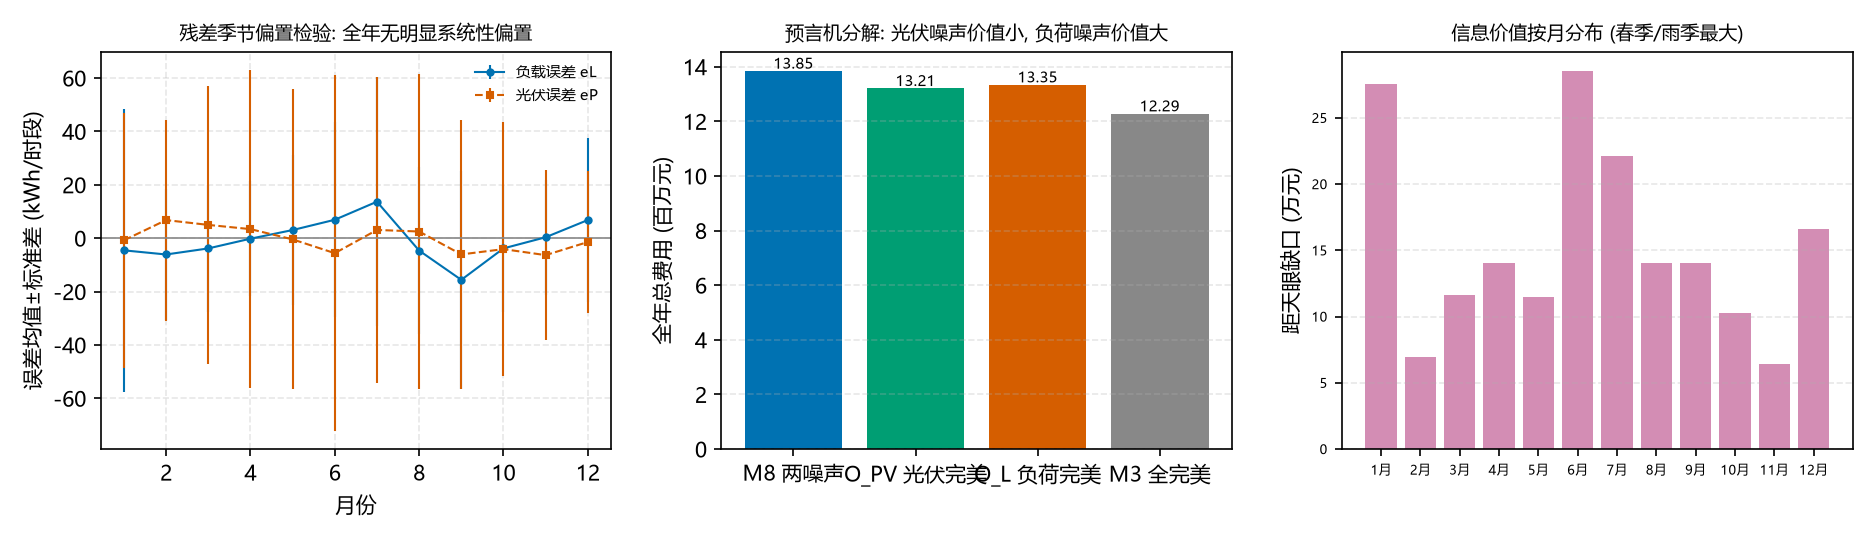
\includegraphics[width=0.95\textwidth]{figures/fig_noise.png}
\caption{噪声与季节性证据：残差逐月均值$\pm$标准差（左）、预言机信息价值分解（中）、
距完全信息下界的缺口按月分布（右）}
\label{fig:noise}
\end{figure}

\begin{figure}[htbp]
\centering
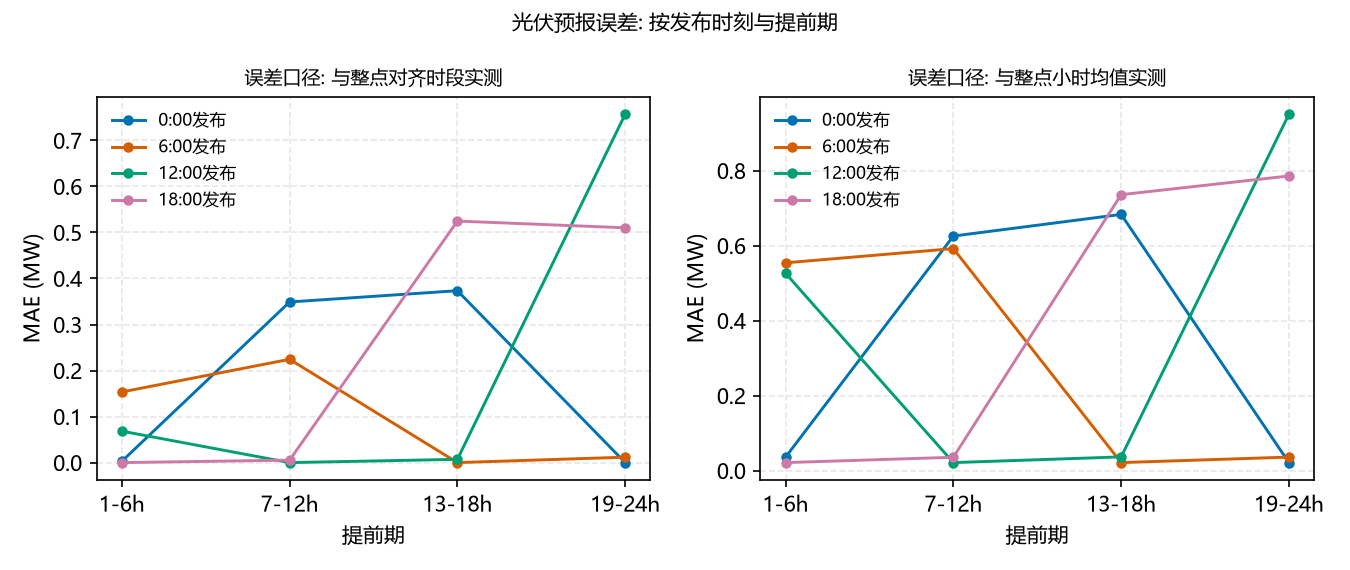
\includegraphics[width=0.85\textwidth]{figures/fig_fcerr.png}
\caption{光伏预报误差：按发布时刻与提前期分桶的平均绝对误差}
\label{fig:fcerr}
\end{figure}

\subsection{规律与建模决策汇总}

\begin{table}[htbp]
\centering
\caption{全部数据规律及其建模决策}
\label{tab:patterns}
\scriptsize
\begin{tabularx}{\textwidth}{@{}p{2.5cm}p{3.6cm}p{2.4cm}X@{}}
\toprule
规律 & 关键数字 & 决策 & 依据/证据 \\
\midrule
周内负荷 & 周五六低 36.8\% & \textbf{已建模并升级}（水平$\times$形状 + 分类凸组合） & 负载 MAE $137.5\to132.3$ kW（周五六 $-8.0\%$），全年 $-36.5\text{\%}$ \\
周内电价 & 周五六低 23.3\% & 不单独建模 & LP 自动利用（周五净充最高）；用预测电价反而 $-0.20\text{\%}$ \\
光伏季节 & 1.93 倍，正弦 $R^2=0.754$，6 月凹陷 & 不单独建模 & 动量修正 $+0.63\text{\%}$；残差无季节偏置；$q^*$ 逐月不变 \\
负荷季节 & 夏高冬低（104--128 MWh/日） & 不单独建模 & 同类日平均残差无季节偏置 \\
噪声重尾 & 峰度 $+5.96$ & \textbf{已建模}（经验分位缓冲） & 复杂缓冲形式差异 $<0.6\text{\%}$；$q=0.5$ 则 $+8.27\text{\%}$ \\
信息价值 & 光伏 35.9\%/负荷 31.0\%/交互 33.2\% & 只做“可实现的改进” & 两项噪声上限 91.5 万，实时平衡已省 90.2 万 \\
预报提前期 & MAE 181$\to$260 kW；更新 273 kW & \textbf{已建模}（滚动调整） & 升级 0:00 依据后调整无正收益（$-28.5\sim+0.3$ 万元） \\
\bottomrule
\end{tabularx}
\end{table}
